\documentclass[12pt,letterpaper,noanswers]{exam}
\usepackage[usenames,dvipsnames,svgnames,table]{xcolor}
\usepackage[margin=0.9in]{geometry}
\renewcommand{\familydefault}{\sfdefault}
\usepackage{multicol}
\pagestyle{head}
\header{AM 111 Class 21}{}{Fast Fourier transform, p.\thepage}
\runningheadrule
\headrule
\usepackage{siunitx}
\usepackage{graphicx} % more modern
\usepackage{amsmath} 
\usepackage{amssymb} 
\usepackage{hyperref}
\usepackage{tcolorbox}
\usepackage{enumitem}
\def\mbf{\mathbf}
\newcommand{\vc}[1]{\boldsymbol{#1}}
\def\dsst{\displaystyle}
\DeclareMathOperator*{\argmin}{arg\,min} % thin space, limits underneath in displays
\usepackage[numbered,autolinebreaks,useliterate]{mcode}

\begin{document}
 \pdfpageheight 11in 
  \pdfpagewidth 8.5in

\noindent 

\section*{Preliminaries}


\begin{itemize}
\itemsep0pt
\item Your out of class assignment this week is project work.
\item There is a skill check in the next class.
\item Sarah's OH are cancelled today - find me on Ed.
\end{itemize}


\noindent\textbf{Big picture}

Today: Decomposing data using sinusoidal functions (Fourier methods).

\vspace{0.2cm}
\hrule
\vspace{0.2cm}

\noindent \textbf{Skill check practice}
\begin{questions}
\item Match the signal to its DFT amplitude.  Provide reasoning.

Signal:

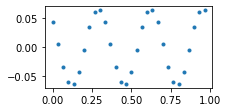
\includegraphics[width=0.3\linewidth]{img/C21skill.png}

Frequency options:

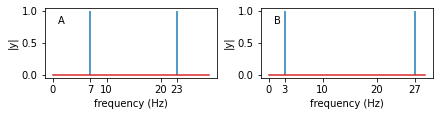
\includegraphics[width=0.7\linewidth]{img/C21skill2.png}


\item The skill from the Class 18 handout (Skill Check C19).
\end{questions}


\vspace{0.2cm}
\hrule
\vspace{0.2cm}

\noindent \textbf{Skill check solution}
\begin{questions}
\item The options for frequency are at 7 Hz or a 3 Hz.  Three sinusoid periods is about right for this signal (definitely not 7 periods).  So option B.
\item See the past handout.
\end{questions}
\vspace{0.2cm}
\hrule
\vspace{0.2cm}

\noindent \textbf{Teams}
\begin{multicols}{3}
1. Mina, Ivonne, Emma

2.  RJ, Johan, Shang

3. Benjamin, Julia K, Dani

4. Nini, Mack, Daniyal

5. Kevin G, Julia M, Nina

6. Jack, Caitlin, Esmé

7. Cameron, Robert, Tom

8. Ray, Alex H, Jessica

9. Eli, Basil, Zachary

10.  Kevin C, Eric, Brian

11. Eletria, Sophia, Aidan

12. Alex B, Nicolas, Marissa

\end{multicols}


\begin{tcolorbox}
A \textbf{discrete Fourier transform} (DFT) allows you to find weights, $y_k$, for the discrete Fourier basis vectors given a signal $\vc{x}$.

 Let $\vc{y} = [y_0, y_1,...,y_{n-1}]^T$.  The \textbf{inverse DFT} allows you to find $\vc{x}$ given the set of weights $\vc{y}$ in frequency space.

\end{tcolorbox}

\begin{tcolorbox}
For a signal that will have $n$ samples, the inverse DFT is given by 
 $\vc{x} = F_n^{-1}\vc{y}.$
 
Let $\vc{w}_n^{(k)} = \frac{1}{n}\left[e^{2\pi i k/n},
e^{2\pi i 2k/n},
\hdots, 
e^{2\pi i (n-1)/n}\right]^T$ 

$\vc{w}_n^{(k)}$ is the $k$th discrete Fourier basis vector.

We have $F_n^{-1} = \left[\vc{w}_n^{(0)}\  \vc{w}_n^{(1)}\  \hdots\vc{w}_n^{(n-1)}\right]$ and

\[\vc{x} = y_0\vc{w}_n^{(0)} +  y_1\vc{w}_n^{(1)}+...+y_{n-1}\vc{w}_n^{(n-1)}.\]
\end{tcolorbox}

\begin{enumerate}[resume=classQ]
\item The plots below were made by setting $y_k = 0$ for all $k$ except $k=2$.  $y_2 = 1$ for the row with $25$ samples.
\begin{parts}
\item Compare the middle plots ($\text{Re}(x)$ vs $t$).  How do they differ from each other?  What about the plots of $\text{Im}(x)$ vs $t$?
\vspace{1cm}
\item In the top row you are seeing $\text{Re}(\vc{w}_{25}^{(2)})$ and $\text{Im}(\vc{w}_{25}^{(2)})$ in the two plots.  What are you seeing in the bottom row plots?
\vspace{1cm}

\item Sketch how you think $\text{Re}(n\vc{w}_n^{(2)})$ would look for large $n$.  \emph{Include ticks on the axes to show amplitude.}
\vspace{1in}
\end{parts}
\end{enumerate}

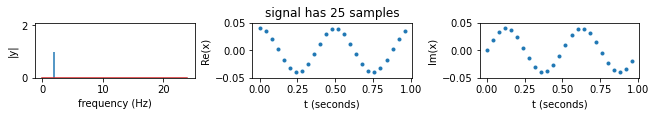
\includegraphics[width=0.9\linewidth]{img/C21ex1a.png}

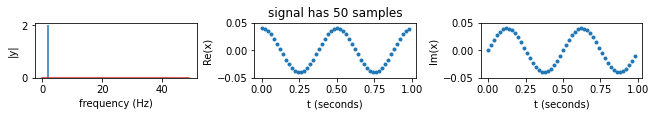
\includegraphics[width=0.9\linewidth]{img/C21ex1.png}



\begin{enumerate}[resume = classQ]
\item Below are plots with $y_{n-2}$ nonzero (where $n = 25$ and $n = 50$ respectively) and all other $y_k = 0$.  How do they differ from the plots above?
\vspace{1in}
\end{enumerate}

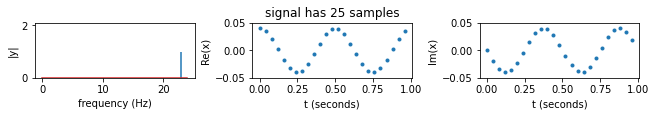
\includegraphics[width=0.9\linewidth]{img/C21ex3a.png}

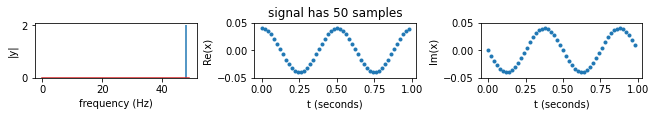
\includegraphics[width=0.9\linewidth]{img/C21ex3.png}



\begin{tcolorbox}
Given a signal generated by sampling a sinusoid at even intervals in time, it is not possible to uniquely determine the frequency of the original sinusoid.  This is called \textbf{aliasing}.  
\end{tcolorbox}

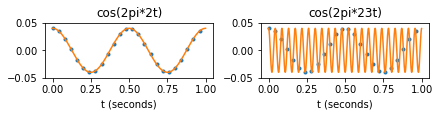
\includegraphics[width=0.7\linewidth]{img/C21alias.png}

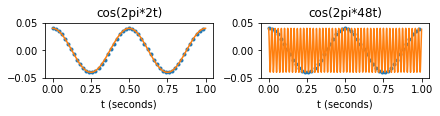
\includegraphics[width=0.7\linewidth]{img/C21alias50.png}

\begin{enumerate}[resume=classQ]
    \item For both $n=25$ and $n=25$, the signal in the plot on the left is at 2 Hz (two periods per second).  What about on the left?
    \vspace{1cm}
\end{enumerate}

\noindent Depending on sampling rate (number of samples per second) a different frequency aliases to $2$ Hz.

\begin{tcolorbox}
For a real valued signal, $\vc{x}$, the amplitude of the frequency spectrum, $\vert\vc{y}\vert$, generated by computing a DFT will be symmetric about a middle frequency, called the \textbf{Nyquist frequency}.

The Nyquist frequency depends on the sampling rate.
\end{tcolorbox}

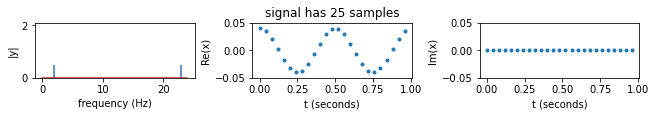
\includegraphics[width=0.9\linewidth]{img/C21ex2a.png}

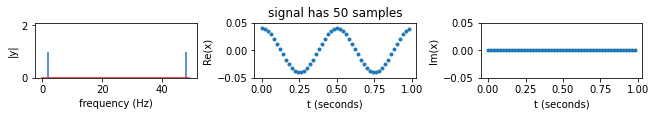
\includegraphics[width=0.9\linewidth]{img/C21ex2.png}



\subsection*{Computing the DFT: the fast Fourier transform (Sauer \S 10.1.3)}

\begin{tcolorbox}
The straightforward way to compute the DFT or inverse DFT involves multiplying an $n\times n$ matrix by a vector and uses $\mathcal{O}(n^2)$ operations.

An algorithm called the \textbf{fast Fourier transform} (FFT) (1965 by Cooley and Tukey) computes the DFT in $\mathcal{O}(n\log n)$ operations.
\end{tcolorbox}

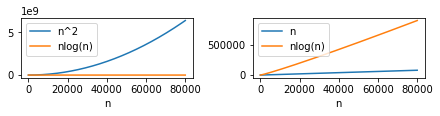
\includegraphics[width=0.7\linewidth]{img/C21dfttime.png}

\noindent\textbf{Example (from Sauer) compute $\vc{y} = F_n \vc{x}$ recursively.:}

  For the $n=4$ case: Set $\omega = e^{-2\pi i/4} = -i$. The DFT is

 \[\vc{y} = \left[\begin{array}{l l l l} \omega^0 & \omega^0 & \omega^0 & \omega^0 \\
\omega^0 & \omega^{1} & \omega^{2} & \omega^{3} \\
\omega^0 & \omega^{2} & \omega^{4} & \omega^{6} \\
\omega^0 & \omega^{3} & \omega^{6} & \omega^{9} \\
\end{array}\right]\vc{x}\]

\noindent In the matrix product, rearrange so even $x_k$ are first and odd are second (note that $\omega^0 = 1$):
\begin{align*}
y_0 &= (\omega^0x_0 + \omega^0x_2) + (\omega^0x_1+\omega^0x_3) \\
y_1 &= (\omega^0x_0 + \omega^2x_2) + (\omega^1x_1+\omega^3x_3) \\
y_2 &= (\omega^0x_0 + \omega^4x_2) + (\omega^2x_1+\omega^6x_3) \\
y_3 &= (\omega^0x_0 + \omega^6x_2) + (\omega^3x_1+\omega^9x_3) \\
\end{align*}

Pull out common factors:

\begin{align*}
y_0 &= (\omega^0x_0 + \omega^0x_2) + \omega^0(\omega^0x_1+\omega^0x_3) \\
y_1 &= (\omega^0x_0 + \omega^2x_2) + \omega^1(\omega^0x_1+\omega^2x_3) \\
y_2 &= (\omega^0x_0 + \omega^4x_2) + \omega^2(\omega^0x_1+\omega^4x_3) \\
y_3 &= (\omega^0x_0 + \omega^6x_2) + \omega^3(\omega^0x_1+\omega^6x_3) \\
\end{align*}
In general, $\omega^n = 1$.  In this case, $\omega^4 = 1$.
\begin{enumerate}[resume=classQ]
\item In the four equations above, for $\omega^k$ with $k>3$, rewrite this as $\omega^{k-4}$.  Notice that some of the quantities in parentheses are now identical.
\vspace{1.5in}
\end{enumerate}

We can write $F_4\vc{x}$ as
\begin{align*}
y_0 &= u_0 + \omega^0v_0 \\
y_1 &= u_1 + \omega^1v_1 \\
y_2 &= u_0 + \omega^2v_0 \\
y_3 &= u_1 + \omega^3v_1 \\
\end{align*}

where $\vc{u} = [u_0\ u_1]^T$, $\vc{v} = [v_0\ v_1]^T$ and $\vc{u} = F_2\left[\begin{array}{c} x_0 \\ x_2 \end{array}\right]$, $\vc{u} = F_2\left[\begin{array}{c} x_1 \\ x_3\end{array} \right]$.

\begin{enumerate}[resume=classQ]
\item Assume that an $F_{2^5}\vc{x}$ calculation can be split into two $F_{2^4}\hat{\vc{x}}$ calculations, and on into $F_2\tilde{\vc{x}}$ calculations:
\begin{parts}
\item How many $F_2\tilde{\vc{x}}$ calculations arise starting from $F_{2^5}\vc{x}$?
\vspace{1cm}
\item How many would arise from $F_{2^m}\vc{x}$?
\vspace{1cm}
\end{parts}
\end{enumerate}

\begin{tcolorbox}
Theorem (10.5 from Sauer \S 10.1.3): Let $n$ be a power of $2$.  The fast Fourier transform of size $n$ can be completed in $n(2\log_2 n-1)+1$ additions and multiplications.
\vspace{0.1cm}

The proof is available in Sauer: you can also think of this as $n = 2^m$ and the FFT of size $2^m$ can be completed in $2^m(2m-1)+1$ additions and multiplications.


\end{tcolorbox}

% The inverse DFT is $\vc{x} = \frac{1}{4}\left[\begin{array}{l l l l} \omega^0 & \omega^0 & \omega^0 & \omega^0 \\
% \omega^0 & \omega^{-1} & \omega^{-2} & \omega^{-3} \\
% \omega^0 & \omega^{-2} & \omega^{-4} & \omega^{-6} \\
% \omega^0 & \omega^{-3} & \omega^{-6} & \omega^{-9} \\
% \end{array}\right]\vc{y}$


% Let $\vc{w}_n^{(k)} = \left[\begin{array}{l}e^{-2\pi i k/n} \\
% e^{-2\pi i 2k/n}\\
% \vdots \\ 
% e^{-2\pi i (n-1)/n}\end{array}\right]
% = 
% \left[\begin{array}{l}\cos(-2\pi \frac{k}{n}) \\
% \cos(-2\pi \frac{2k}{n})\\
% \vdots \\ 
% \cos(-2\pi \frac{n-1}{n})\end{array}\right]
% + i \left[\begin{array}{l}\sin(-2\pi \frac{k}{n}) \\
% \sin(-2\pi \frac{2k}{n})\\
% \vdots \\ 
% \sin(-2\pi \frac{n-1}{n})\end{array}\right]
% = 
% \left[\begin{array}{l}\cos(2\pi \frac{k}{n}) \\
% \cos(2\pi \frac{2k}{n})\\
% \vdots \\ 
% \cos(2\pi \frac{n-1}{n})\end{array}\right]
% - i \left[\begin{array}{l}\sin(2\pi \frac{k}{n}) \\
% \sin(2\pi \frac{2k}{n})\\
% \vdots \\ 
% \sin(2\pi \frac{n-1}{n})\end{array}\right]
% $


% \begin{tcolorbox}
% \begin{itemize}
% \itemsep0pt
%      \item The DFT is given by
     
%     \[\vc{y} =F_n\vc{x}\] where
%     \[F_n =  \left[\begin{array}{l l l l l}
%     \omega^0 & \omega^0 &\omega^0 & \hdots & \omega^0 \\
%     \omega^0 & \omega^{1} & \omega^{2} & \hdots & \omega^{n-1} \\
%     \omega^0 & \omega^{2} & \omega^{4} & \hdots & \omega^{2(n-1)}\\
%     \vdots & \vdots & \vdots & & \vdots \\
%     \omega^0 & \omega^{n-1} & \omega^{2(n-1)} & \hdots &\omega^{(n-1)^2}
%     \end{array}\right]\]
%     and  $\omega = e^{-2\pi i/n} = \cos(2\pi/n) - i\sin(2\pi/n)$.
%     \item 
%     %From $\vc{x} = \sum\limits_{k=0}^{n-1}y_k \vc{w}_n^{(k)}$, 
%     The inverse DFT is given by 
%  \[\vc{x} = F_n^{-1}\vc{y}\]
%  where \[F_n^{-1} = \dfrac{1}{n} \left[\begin{array}{l l l l l}
%     \omega^0 & \omega^0 &\omega^0 & \hdots & \omega^0 \\
%     \omega^0 & \omega^{-1} & \omega^{-2} & \hdots & \omega^{-(n-1)} \\
%     \omega^0 & \omega^{-2} & \omega^{-4} & \hdots & \omega^{-2(n-1)}\\
%     \vdots & \vdots & \vdots & & \vdots \\
%     \omega^0 & \omega^{-(n-1)} & \omega^{-2(n-1)} & \hdots &\omega^{-(n-1)^2}
%     \end{array}\right]\]
% %  %\left[\vc{w}_n^{(0)}, \vc{w}_n^{(1)},...,\vc{w}_n^{(n-1)}\right]\vc{y}\]
% %  \item $\vc{w}_n^{(k)} = \dfrac{1}{n}\left[\omega^{0k}, \omega^{-k}, \omega^{-2k}, \omega^{-3k},...,\omega^{-(n-1)k}\right]^T$ 
  
% \end{itemize}
% The choice of how to incorporate the factor $1/n$ is not standardized.  For example, it is sometimes split as a factor of $1/\sqrt{n}$ on both $F_n$ and $F_n^{-1}$.  The choice above is made to match \texttt{scipy.fft}.
% \end{tcolorbox}


% \begin{enumerate}[resume=classQ]
%     \item That $F_n^{-1}$ is the inverse of $F_n$ is not obvious.  Let $a_{jk}$ be the $(j,k)$ entry in $F_n^{-1}F_n$.
%     \begin{parts}
%     \item Consider the diagonal entries, $a_{kk}$.  These are given by \[\dfrac{1}{n}\left[\omega^0, \omega^{-k},\omega^{-2k},\hdots,\omega^{-k(n-1)}\right]\left[\begin{array}{l}
%     \omega^0\\
%     \omega^{k}\\
%     \omega^{2k}\\
%     \vdots\\
%     \omega^{k(n-1)}
%     \end{array}\right]\]
    
%     Show that the diagonal terms are $1$.
%     \vspace{1in}
    
%     \item Now we need to show that the off-diagonal terms are $0$.  
    
%     \[\dfrac{1}{n}\left[\omega^0, \omega^{-j},\omega^{-2j},\hdots,\omega^{-j(n-1)}\right]\left[\begin{array}{l}
%     \omega^0\\
%     \omega^{k}\\
%     \omega^{2k}\\
%     \vdots\\
%     \omega^{k(n-1)}
%     \end{array}\right]\]
    
%     Find an appropriate $c$ and write this as $\dfrac{1}{n}\left(1 + \omega^{c}+\omega^{2c} + ... + \omega^{c(n-1)}\right)$.
%     \vspace{1cm}
%     \item $\omega$ is the $n$th root of unity.  Use Euler's formula ($e^{ix} = \cos x + i\sin x$) to convince yourself that $\omega^n = 1$.
%     \vspace{1cm}
%     \item For $1\leq c < n$, show that
%     $(1-\omega^c)(1+\omega^c + \omega^{2c} + \omega^{3c} + ... + \omega^{c(n-1)}) = 1-\omega^{cn}$.
%     \vspace{1in}
%     \item Given that $\omega^n = 1$, $\omega^{cn} = 1$, and $\omega^c \neq 1$, what can you conclude about $1+\omega^c + \omega^{2c} + \omega^{3c} + ... + \omega^{c(n-1)}$?
%     \vspace{1in}
    
%     \end{parts}
% \end{enumerate}



\subsection*{DFT and interpolation (Sauer \S 10.2)}
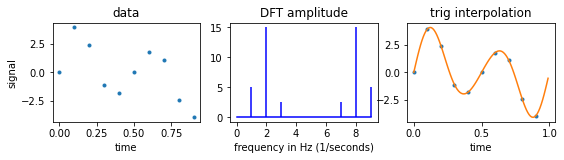
\includegraphics[width=0.8\linewidth]{img/C20interp.png}
\begin{tcolorbox}
\begin{itemize}
\itemsep0pt
    \item Let $\vc{x}$ be real-valued data sampled at evenly spaced points $\vc{t}$ on the interval $[0,1)$, with sample points $t_j = j/n$ for $j=0,...,n-1$.
    \item Let $\vc{y}$ be the DFT of the data.  $\vc{x} = F_n^{-1}\vc{y}$: the sum of the Fourier modes (using weights $\vc{y}$) passes through the data points exactly.
\end{itemize}
\end{tcolorbox}
% \begin{enumerate}[resume=classQ]
% \item For the data in the plot above, the $y_k$ are given by $\vc{y} = \left[\begin{array}{r} 0 \\-5i, \\-15i\\ -2.5i\\ 0\\ 0\\ 0\\ -2.5i\\ -15i\\ -5i\end{array}\right]$
% \begin{parts}
% \item At a frequency of $1$ (a single period in the interval $[0,1)$, $y_1 = -5i$.  The associated trigonometric function is $\frac{1}{10}\cos (2\pi t)+i\sin(2\pi t)$.

% \end{parts}
% \end{enumerate}
\begin{enumerate}[resume=classQ]
\item We let $t_j = j/n$ for $j=0,...,n-1$, so we have $\vc{x} 
% %\sum\limits_{k=0}^{n-1} y_k \frac{1}{n}\left[\begin{array}{l} \omega^0 \\\omega^{-k} \\\omega^{-2k}\\
% \vdots \\
% \omega^{-k(n-1)}\end{array}\right] 
= \sum\limits_{k=0}^{n-1} y_k \frac{1}{n}\left[\begin{array}{l} e^{2\pi i (0/n)} \\e^{2\pi ki (1/n)} \\e^{2\pi ki (2/n)}\\
\vdots \\
e^{2\pi ki ((n-1)/n)}\end{array}\right] = \sum\limits_{k=0}^{n-1} y_k \frac{1}{n}\left[\begin{array}{l} e^{2\pi ki t_0} \\e^{2\pi ki t_1} \\e^{2\pi ki t_2}\\
\vdots \\
e^{2\pi ki t_{n-1}}\end{array}\right]$
\begin{parts}
\item Think of the vector $\vc{w}_n^{(k)} = \frac{1}{n}\left[\begin{array}{l} e^{2\pi ki t_0} \\e^{2\pi ki t_1} \\e^{2\pi ki t_2}\\
\vdots \\
e^{2\pi ki t_{n-1}}\end{array}\right]$ as a complex-valued function, $g_k(t)$, evaluated at the time points $\vc{t}$.  Write down $g_k(t)$.
\vspace{1cm}
\item Let $y_k = a_k + i b_k$.  Find the real part of $(a_k + ib_k)g_k(t)$.
\vspace{0.8in}
\item The real function $P(t)$, given by the real part of $\sum\limits_{k=0}^{n-1} y_kg_k(t)$, uses the weights $y_k$ as interpolation coefficients on trig functions.  Use your result from (b) to write an expression for $P(t)$.
\vspace{0.7in}
\end{parts}
\end{enumerate}

\subsection*{(extra fact) DFT and least squares (Sauer \S 10.3.2)}
\begin{tcolorbox}
\begin{itemize}
\itemsep0pt
    \item Consider the trigonometric least squares problem, where $m$ basis functions (with indices $S = \{j_0,j_2,...,j_{m-1}\}$) are chosen for least squares fitting from the $g_k(t)$ above.
    \item For $m<n/2$, this is a compression problem.
    \item $P_m(t) = \sum\limits_{k=0}^m y_{j_k}g_{j_k}(t)$.  The error vector, $\vc{e} = P(\vc{t}) - P_m(\vc{t}) = \sum\limits_{k\notin S}y_k g_k(\vc{t})$.  The vectors formed by $g_k$ evaluated at $\vc{t}$ are orthogonal, so $\vc{e}$ is orthogonal to the span of $\left\{g_{j_k}(\vc{t})\right\}_{j_k\in S}$.  i.e. $P_m(t) = \sum\limits_{k=0}^m y_{j_k}g_{j_k}(t)$ is the least squares solution.
\end{itemize}
\end{tcolorbox}
\end{document}